% \chapter{Implementation Tools}%
% \label{chapter:tools}

% As defined earlier in section~\ref{section:Goals}, the primary goal of this dissertation is to leverage the Human-Robot Collaboration \ac{HRC} paradigm by integrating \ac{MR} technologies alongside robot capabilities to enhance remote collaboration. In order to achieve this, a conceptual model is further implemented.

% \section{Conceptual Model}
% In order to start addressing the mentioned challenges, a first effort has been made. A robotic arm from Universal Robots, UR10e, shown in the figure \ref{f:ur10e_iris}, available at IRIS LAB, was used as a dynamic agent to assist in shared activities.
% %  add a footnote to the robot model in universal robots website

% \begin{figure}[h]
%     \centering
%     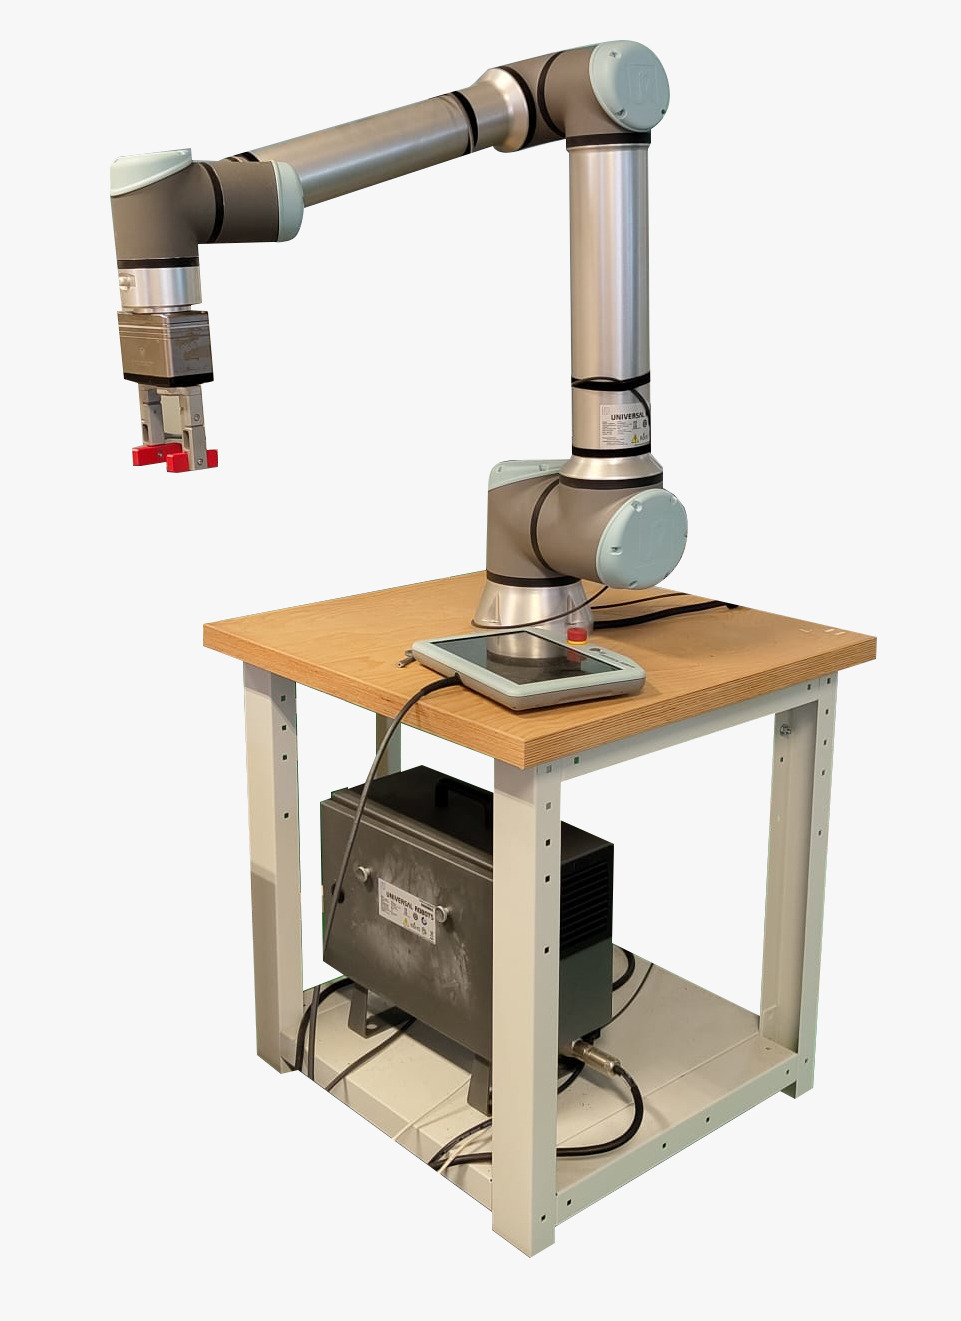
\includegraphics[width=0.4\linewidth]{figs/ur10e.jpeg}
%     \caption{Robot UR10e used for the development of the dissertation work, available at IRIS-LAB, University of Aveiro}
%     \label{f:ur10e_iris}
% \end{figure}



% \section{Digital Model Implementation of the Robot}
% \label{section:digital-model}

% \subsection{Unity}

% Unity is a dynamic and versatile game engine developed by Unity Technologies \footnote{Unity Technologies \url{https://unity.com/} Accessed: 2024-09-30}, widely recognized for revolutionizing game development over the past few years. Beyond gaming, it has become a prominent tool for creating \ac{AR}, \ac {VR}, and \ac{MR} applications. Its user-friendly interface empowers developers to rapidly craft immersive experiences while simplifying complex development processes.

% By offering an \ac{IDE} that combines \ac{GUI} manipulation of scene objects with a code editor, similar to Visual Studio, it allows developers to build virtual scenes by either creating or integrating 2D and 3D assets as well as apply attributes such as lighting, audio, physics properties, animations, and interactive gameplay logic. Afterwards, these composed scenes come to life, rendering them in real-time at frame rates that create smooth motion and immersive experiences.

% One of Unity's significant advantages is its extensive platform compatibility. It supports development for various operating systems, including Windows, and Linux, as well as mobile platforms like iOS and Android. Additionally, a wide range of devices spanning \ac{AR},\ac{VR},\ac{MR} technologies are supported.

% Unity's choice for developing the \ac{MR} application was advised by both supervisors regarding its versatility as well as its robust capabilities and extensive feature set.

% \subsection{Digital Robot Model - URDF Importer Package}
% % % % foi necessário encontrar um modelo do robot a ser utilizado - UR10e que se encontra no IRIS lab
% To successfully develop the XR application for controlling the UR10e robot, it was essential to identify a model that closely mirrors 
% the actual robot. The Unity Robotics Hub \footnote{Unity Technologies \url{https://github.com/Unity-Technologies/Unity-Robotics-Hub} 
% Accessed: 2024-02-02} facilitates the integration of robotics into Unity projects via the URDF-Importer package 
% \footnote{Unity Technologies \url{https://github.com/Unity-Technologies/URDF-Importer} Accessed: 2024-02-02}. 
% However, challenges arose when attempting to import the UR10e \textit{.urdf} model into the Unity environment. To overcome this, 
% a UR10 model, sourced from a GitHub repository \footnote{PositronicsLab \url{https://github.com/PositronicsLab/reveal_packages/tree/master/industrial_arm/scenario/models/urdf/ur10} Accessed: 2024-02-05} 
% was used, due to its resemblance to the UR10e robot. This was discussed with the educators overseeing the dissertation development, 
% and it was agreed that this approach would not pose any issues.

% In the figure \ref{f:ur10_marker_unity} it is possible to see the digital UR10 model positioned related to the aruco marker 
% (\ref{f:aruco_marker}), in a simulated Unity environment.
% \begin{figure}[h]
% \centering
% 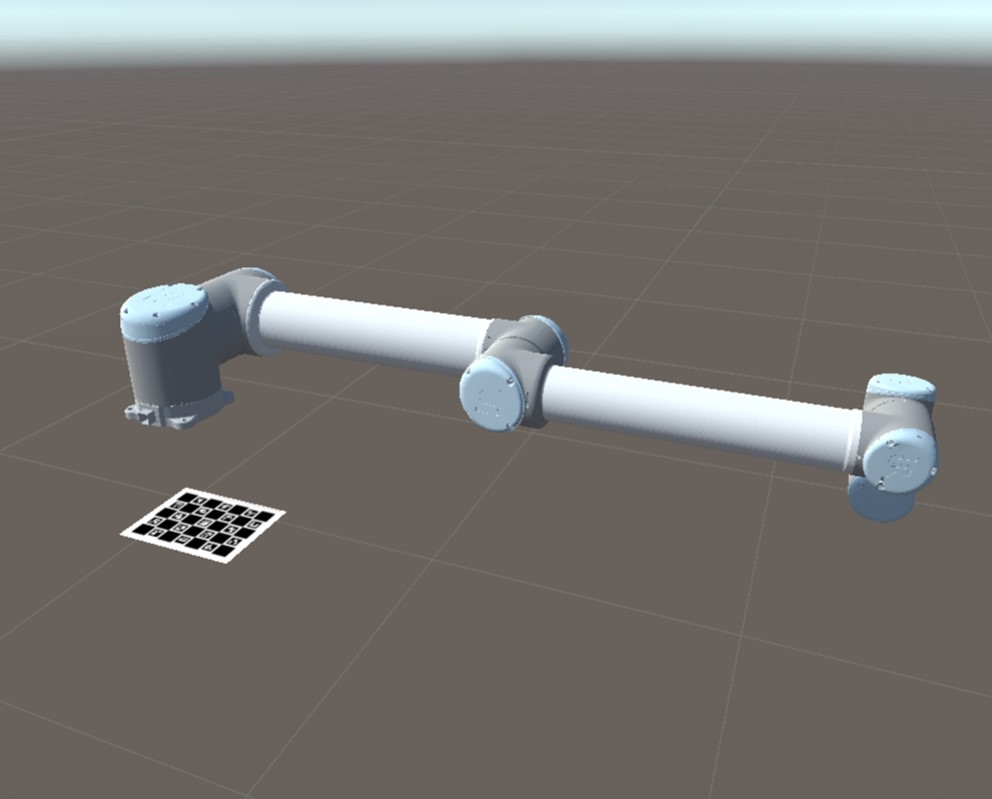
\includegraphics[width=0.6\textwidth]{figs/robot_marker_unity.jpg}
% \caption{Digital UR10 model related to the aruco marker, on Unity environment}
% \label{f:ur10_marker_unity}
% \end{figure}
 - commented this part because text is below - choose whether to use this or the text below

%     % foi necessário encontrar um modelo do robot a ser utilizado - UR10e que se encontra no IRIS lab
%     To successfully develop the \ac{MR} application for controlling the UR10e robot, it was essential to identify a model that closely mirrors 
%     the actual robot. The Unity Robotics Hub \footnote{Unity Robotics Hub \url{https://github.com/Unity-Technologies/Unity-Robotics-Hub} 
%     Accessed: 2024-02-02} facilitates the integration of robotics into Unity projects via the URDF-Importer package 
%     \footnote{Unity URDF Importer \url{https://github.com/Unity-Technologies/URDF-Importer} Accessed: 2024-02-02}. 
    
%     However, instead of importing the UR10e \textit{.urdf} model into the Unity environment, a UR10 model, sourced from a GitHub repository \footnote{PositronicsLab \url{https://github.com/PositronicsLab/reveal_packages/tree/master/industrial_arm/scenario/models/urdf/ur10} Accessed: 2024-02-05} 
%     was used, due to its resemblance to the UR10e robot. 
%     % This was discussed with the educators overseeing the dissertation development, and it was agreed that this approach would not pose any issues.


% % \ac{MR} alongside a static robotic arm (UR10e) to support remote collaboration scenarios. This involves transforming human-robotic collaboration by integrating \ac{MR} technologies and robotic capabilities to enhance both on-site and remote collaboration experiences.

% % Unity 3D engine will allow robot model development, enabling detailed and interactive digital twins with bilateral communication capabilities. By utilizing Vuforia for precise pose registration, the system ensures accurate spatial alignment between the virtual and physical robots.

% % To enhance user awareness and prevent accidents, the system will implement visual and audio cues within the \ac{AR} environment, including safety-zone interactions and audio alerts. These features provide intuitive feedback to users, improving situational awareness during human--robot collaboration. The robot manipulation interface will be designed to be user-friendly, allowing non-expert users to operate the robot remotely using a handheld device (\ac{HHD}). This accessibility ensures that a wider range of users can effectively interact with the robotic system without extensive training.

% % Real-time updates of the robot's position and workspace visualization will be provided through camera feed transmission, offering remote users a comprehensive view of the operational environment. This feature addresses the limitations identified in existing literature, where remote users often lack sufficient context and visibility of the workspace.

% % % Furthermore, the proposed system will address challenges identified in the state-of-the-art review, such as networking latency and positioning accuracy. By implementing optimized communication protocols and advanced tracking algorithms, the system aims to ensure efficient and safe human--robot collaboration. These improvements will not only enhance the performance of the system but also contribute valuable insights to the field, bridging the gap between on-site and remote interaction capabilities in industrial applications.

% % Overall, this project seeks to expand upon current research by providing a holistic solution that integrates advanced technologies to facilitate seamless collaboration between humans and robots, regardless of physical location. By focusing on both on-site and remote users, the system aims to enhance flexibility, safety, and efficiency in various industrial scenarios.

% \section{Pose registration}

% After having successfully imported the \ac{URDF} model of the real robot into the Unity environment, the next step was to ensure that the digital model was accurately aligned with the physical robot. 

% \subsection{Vuforia}
% \label{section:marker-detection}
% % 
% Vuforia is a software platform that enables the creation of \ac{ar} experiences. 
% % Integrated with Unity, a leading platform for developing games and interactive applications, Vuforia simplifies the incorporation 
% of AR into mobile and digital apps. 
% It uses computer vision technologies to recognize and track images and objects in the real world, allowing developers to overlay digital 
% content precisely.

% The marker illustrated in Figure \ref{f:aruco_marker} was selected following initial attempts that yielded inconsistent results when using 
% the laptop's camera, shown in the figure \ref{fig:camera-c922}, to scan the environment. This particular marker demonstrated greater stability, 
% enabling the precise positioning of the digital UR10 model in alignment with the physical surroundings. Consequently, this facilitated the accurate 
% overlay of the digital UR10 model onto the actual UR10e robot, enhancing the integration of virtual and real-world elements.

% \begin{figure}[h]
%     \centering
%       \begin{subfigure}[b]{0.45\textwidth}
%       \centering
%       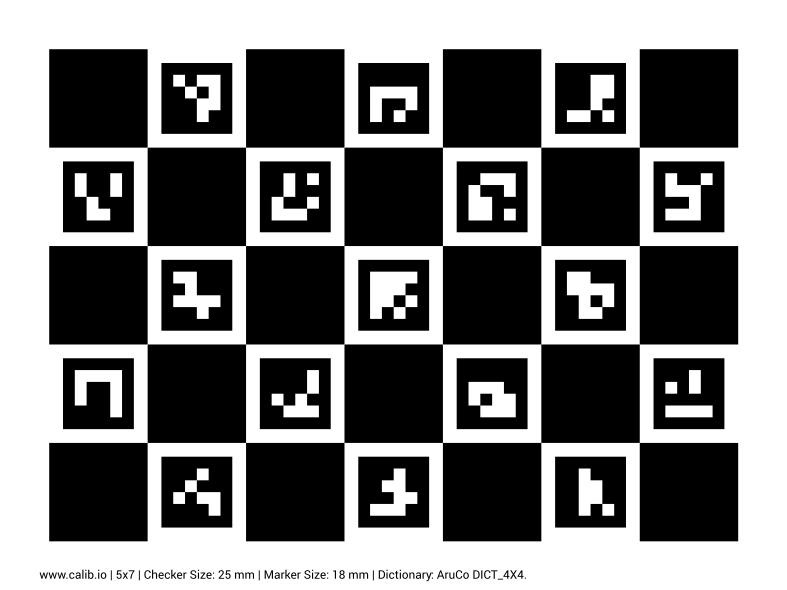
\includegraphics[width=0.7\textwidth]{figs/calib_io_charuco_200x150_5x7_25_18_DICT_4X4.png}
%       \caption{ArUco marker used to allow the segmentation for aligning the digital twin accordingly to the real environment}
%       \label{f:aruco_marker}
%       \end{subfigure}
%         \hfill % This command adds space between the subfigures
%       \begin{subfigure}[b]{0.45\textwidth}
%           \centering
%           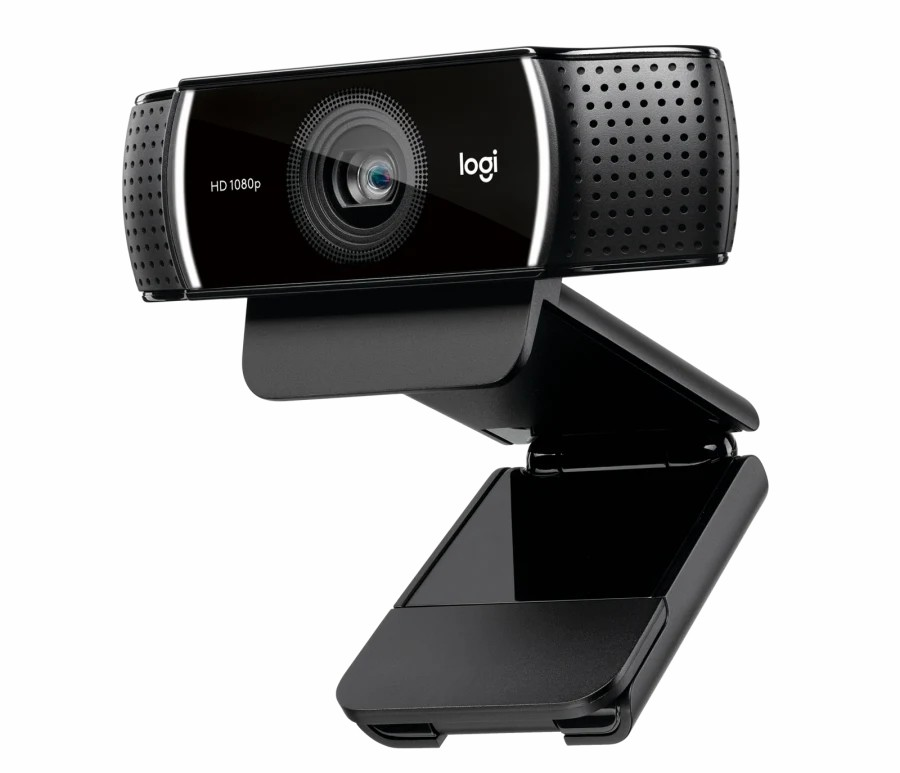
\includegraphics[width=0.7\linewidth]{figs/camera-c922.jpg}
%           \caption{Logitech c922 camera, used for testing on-site application developments}
%           \label{fig:camera-c922}
%       \end{subfigure}
%       \caption{ArUco marker used with the Logitech c922 camera for segmentation and manipulation of virtual environment}
%   \label{marker-camera}
%   \end{figure}
   commented this part because text is below - choose whether to use this or the text below

% This alignment was achieved by utilizing Vuforia, a software platform that enables the creation of \ac{AR} experiences. Integrated with Unity, Vuforia simplifies the incorporation of \ac{AR} into mobile and digital apps. It uses computer vision technologies to recognize and track images and objects in the real world, allowing developers to overlay digital content precisely.

% \subsection{Marker Detection}

% The marker illustrated in Figure \ref{f:aruco_marker}, demonstrated greater stability, enabling the precise positioning of the digital UR10 model in alignment with the physical surroundings. Its choice followed initial attempts that yielded inconsistent results while using some other ArUco generated examples \footnote{ArUco Markers Generator \url{https://chev.me/arucogen/} Accessed: 2024-09-30}. 

% To scan the physical environment around the robot, the camera shown in the figure \ref{fig:camera-c922} was used throughout the features' development process. 

% \begin{figure}[h]
%     \centering
%     \begin{subfigure}[b]{0.45\textwidth}
%     \centering
%     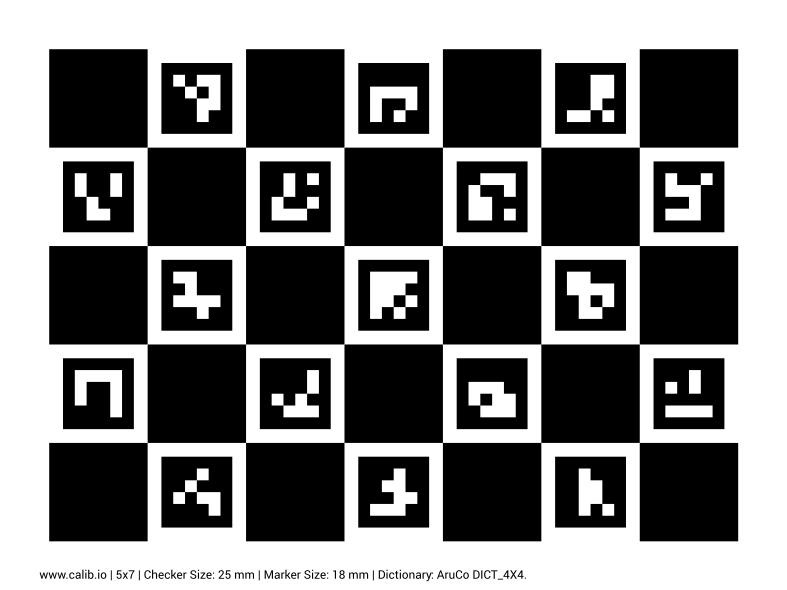
\includegraphics[width=0.7\textwidth]{figs/calib_io_charuco_200x150_5x7_25_18_DICT_4X4.png}
%     \caption{ArUco marker used to allow the segmentation for aligning the digital twin accordingly to the real environment}
%     \label{f:aruco_marker}
%     \end{subfigure}
%         \hfill % This command adds space between the subfigures
%     \begin{subfigure}[b]{0.45\textwidth}
%         \centering
%         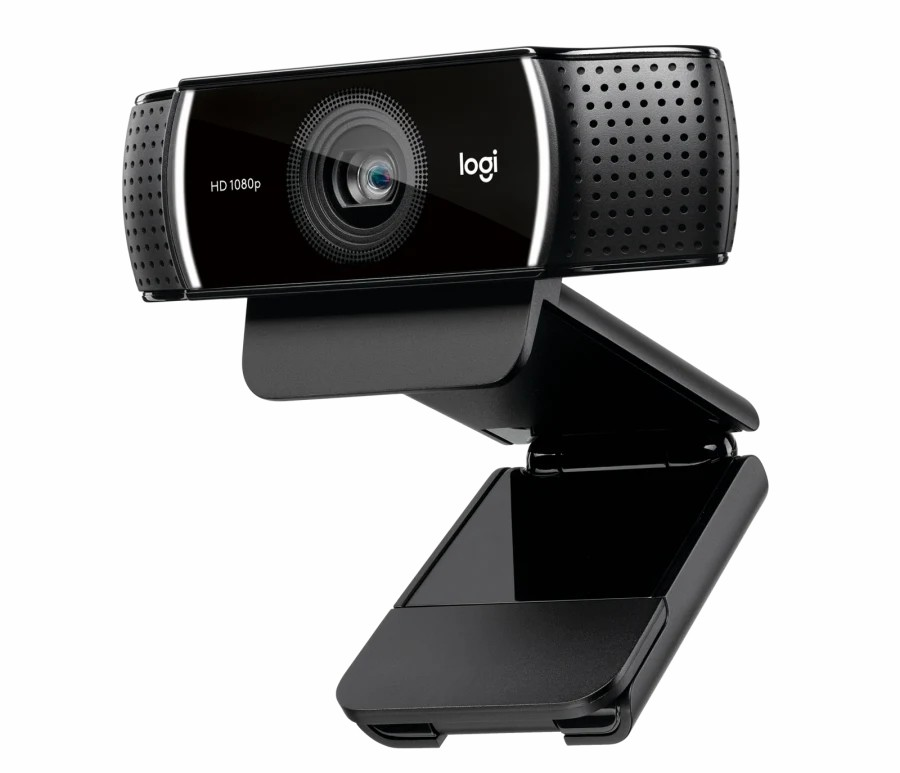
\includegraphics[width=0.7\linewidth]{figs/camera-c922.jpg}
%         \caption{Logitech c922 camera, used for on-site integration}
%         \label{fig:camera-c922}
%     \end{subfigure}
%     \caption{ArUco marker used with the Logitech c922 camera for segmentation and manipulation of virtual environment}
% \label{marker-camera}
% \end{figure}

% Consequently, both the ArUco marker and the Logitech c922 camera allowed to overlay the digital UR10 model on top of the physical robot.
% % enhancing the integration of virtual and real-world elements - use???????

% In the figure \ref{f:ur10_marker_unity} it is possible to see the digital UR10 model positioned related to the aruco marker. 
%     (\ref{f:aruco_marker}), in a simulated Unity environment.
%     \begin{figure}[h]
%     \centering
%     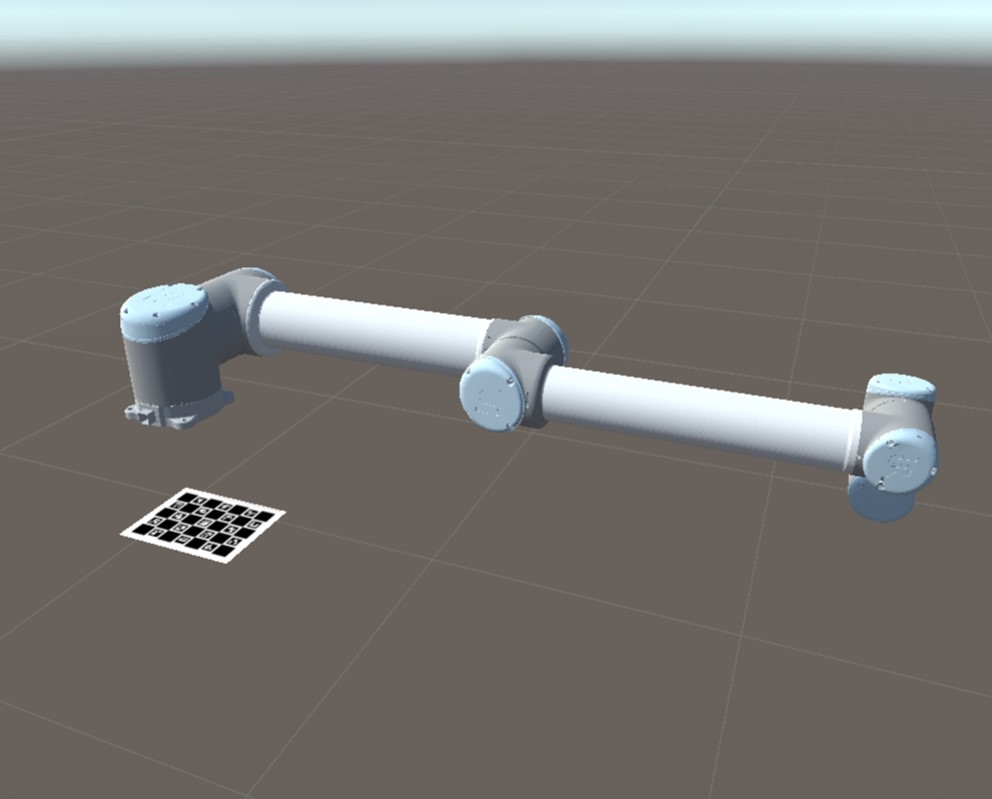
\includegraphics[width=0.6\textwidth]{figs/robot_marker_unity.jpg}
%     \caption{Digital UR10 model related to the aruco marker, on Unity environment}
%     \label{f:ur10_marker_unity}
%     \end{figure}

% \section{Billateral Communication}

% \subsection{UR10e ROS Documentation}
% Unity was chosen for its interactive capabilities, but this choice introduced additional complexity due to the need to operate across different operating systems—Windows for Unity and Ubuntu 20.04 for ROS Noetic, the version supporting the required ROS packages.

% A key advantage was the existence of pre-existing resources from the IRIS Lab, where the robot is housed. Specifically, there were two GitHub repositories—\href{https://github.com/iris-ua/iris_sami}{iris\_sami} and \href{https://github.com/iris-ua/iris_ur10e}{iris\_ur10e}. These provided a well-established ROS environment, enabling control of the UR10e robot through RViz, trajectory planning, and real-time execution. \texttt{iris\_ur10e} package is integral to operating the physical robot in the lab, while \texttt{iris\_sami} allows for the robotic arm's manipulation.

% Given this existing ROS setup on Ubuntu 20.04, ROS-TCP-Connector and ROS-TCP-Endpoint packages from the Unity Robotics Hub (\href{https://github.com/Unity-Technologies/ROS-TCP-Connector}{Unity-Technologies/ROS-TCP-Connector}) were used to establish the Wi-fi Connection. 

% The proposed framework for both laptops connection is shown in figure. (add a figure of the framework proposed).


% % Selecting this package over other ROS-Unity bridges was recommended by João Alves, one of the instructors who provided valuable insights during the development of this project.


% \subsection{Message Generation}

% By having already established the communication between Unity and ROS, specific types of messages from ROS environment had to be exchanged between the network, therefore enabling the robot to be controlled remotely.

% After understanding that the ROS topic responsible for publishing the current state of the robot's joints was \texttt{/joint\_states}, these data needed to be sent to Unity. By adapting the already existing Unity Robotics Hub packages, these messages were not only successfully exchanged between the two environments, but also saved into a \texttt{.json} file for further manipulation.







%%%%%%%%%%%%%%%%%%%%%%%%%%%%%%%%%%%%%%%%%%%%%%%%%%%%%%%%%%%%%%%%%%%%%%%%%%%% 
% from chatgpt - see it and check whether it makes sense or not the use this part instead of the above one (previous version of it)

introduction to implementation tools, unity game engine, vuforia for pose registration, urdf importer for unity, robot operating system, aruco marker for robot alignment, networking and protocols, conclusion

The chapter will explore each tool in detail, providing a thorough explanation of its selection, its integration within the project, and its contribution to the broader \ac{MR}-based \ac{HRC} framework.

\chapter{Implementation Tools}%
\label{chapter:tools}

Achieving the successful integration of Human-Robot Collaboration (\ac{HRC}) and Mixed Reality (\ac{MR}) technologies requires a careful selection of advanced tools, spanning both software and hardware domains. The goal of this dissertation is to construct a robust \ac{MR}-based \ac{DT} framework that allows real-time, remote collaboration and bi-directional robot control. The implementation of such a system introduces several key challenges, including the alignment of physical and digital entities, real-time data communication, and the creation of immersive, user-friendly interfaces. This chapter systematically introduces the key implementation tools used throughout the development of the project, explaining their roles in addressing these challenges. 
The tools discussed in this chapter were chosen for their specific contributions to the project’s overall goal. 

\section{UR10e Robot}

In order to start adressing the aforementioned challenges, a first effort has been made. A robotic arm from Universal Robots, UR10e, shown in the figure \ref{f:ur10e_iris}, available at IRIS LAB.

\begin{figure}[h]
    \centering
    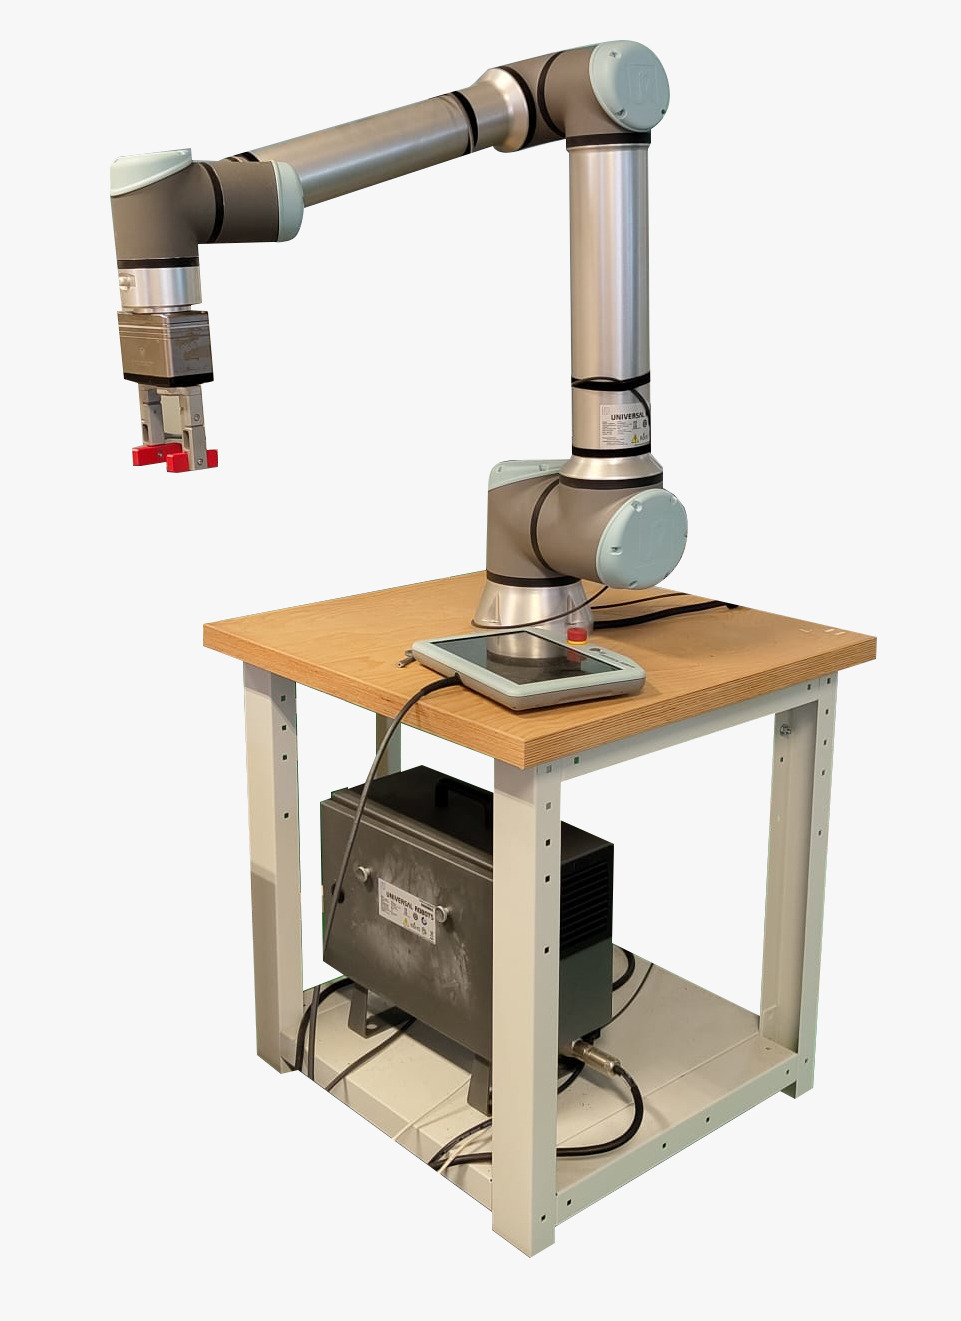
\includegraphics[width=0.4\linewidth]{figs/ur10e.jpeg}
    \caption{UR10e Robot used in the IRIS-LAB, University of Aveiro}
    \label{f:ur10e_iris}
\end{figure}

The UR10e model is one of Universal Robots' most advanced cobots, featuring a payload capacity of 12.5 kg, and a reach of 1300 mm, being designed to automate a wide range of tasks that typically require human input, such as assembly, packaging, and pick-and-place operations \footnote{UR10e \url{https://www.universal-robots.com/products/ur10-robot/} Accessed: 2024-10-15}.

UR10e's integrated force sensors and collision detection technologies allow to collaborate safely with humans in shared workspaces, making it ideal for \ac{HRC} scenarios. Besides, it offers significant flexibility in terms of programming and adaptability. Its console is intuitive and allows imported pre-programmed scripts, therefore being easily deployed across various industrial tasks with minimal programming experience required by the operator.

This robot, as the core physical entity in this human-robot collaborative system, serves as the dynamic agent for performing collaborative tasks, where its physical attributes were mirrored in an immersive digital environment, regarding the fundamental \ac{DT} concept.

\section{Simulation Environment}

\subsection{Unity}

Unity, developed by Unity Technologies, was selected as the primary platform for developing the \ac{MR} environment in this project. Originally designed for game development, Unity has evolved into a powerful tool for creating interactive 3D applications, including \ac{AR}, \ac{VR}, and \ac{MR}. Its robust architecture and versatility in rendering complex virtual environments make it an ideal choice for building a dynamic \ac{DT} of the UR10e robotic arm. This ability to seamlessly integrate external data sources, such as sensor inputs from real-world hardware, enables a high degree of interactivity and realism in the simulation.

Unity’s integrated development environment (\ac{IDE}) allows for rapid prototyping and iterative design of both the virtual space and the \ac{MR} user interface. Moreover, the engine's cross-platform compatibility supports a range of devices, including desktop systems and mobile platforms, and can handle real-time rendering of high-fidelity 3D models, essential for \ac{MR} applications. 
Through the Unity-based simulation, operators can not only control the physical UR10e robot remotely but also visualize real-world tasks in a digital, augmented environment, ensuring accurate synchronization between physical and virtual realms.

In addition, Unity’s robust asset management and scripting support, primarily through C\#, provide developers with the tools to easily simulate complex environments, manage interactive objects, and implement advanced functionality such as collision detection and user input handling. These features enable a realistic and immersive experience for both on-site and remote users, improving the overall effectiveness of the \ac{HRC} system.

% \subsection{Digital Model Implementation of the Robot}

% Here, you can explain how the **Unity URDF Importer package** facilitated the import and management of the robot’s digital model, enabling the creation of a precise digital twin. This section should delve into the **Unity Robotics Hub**, explain why this package was selected, and describe how it contributed to the simulation of the UR10e’s movements and the development of bi-directional communication between the physical and digital environments.


% As introduced in section~\ref{section:Goals}, the primary objective of this dissertation is to explore and implement the concept of Human-Robot Collaboration (\ac{HRC}) by leveraging Mixed Reality (\ac{MR}) technologies. To achieve this goal, a comprehensive framework integrating hardware and software components is designed, facilitating remote collaboration in real-time. This chapter outlines the critical tools used in the implementation of the digital twin, as well as the hardware and software resources required for bi-directional robot control.



\section{Digital Model Implementation of the Robot}
\label{section:digital-model}

\subsection{Digital Robot Model - URDF Importer Package}
In order to correctly mirror the UR10e physical robot model and establish a functional \ac{DT} bidirectional synchronization, the (\ac{URDF}) model of the robot was imported to Unity simulation environment. Unity Robotics Hub's \ac{URDF} Importer package was used for this very purpose \footnote{Unity Robotics Hub \url{https://github.com/Unity-Technologies/Unity-Robotics-Hub} Accessed: 2024-02-02}.
This package provided several key advantages during the implementation of the \ac{DT} for the UR10e robot.

The \textit{Unity \ac{URDF} Importer} package significantly facilitated the integration of the \ac{URDF} file, enabling the precise recreation of the UR10e robot's physical structure, including its joints and linkages. This seamless integration supported real-time simulation of the robot's movements and configurations within the \ac{Unity} environment. Additionally, it allowed the visualization and fine-tuning of physics properties to accurately reflect the robot's real-world dynamics. Essential for bilateral communication between virtual and physical robots, the package also streamlined sensor data import from \ac{ROS}, enhancing the realism of simulations and optimizing development and testing processes.

\section{Pose Registration}
Pose registration is a crucial step in aligning the digital model with the physical robot. In this project, Vuforia, a cutting-edge \ac{AR} software platform, was integrated with Unity to accomplish this alignment.

\subsection{Vuforia}
\label{section:marker-detection}

Vuforia, a powerful \ac{AR} platform, offers robust object recognition and tracking solutions, crucial for \ac{MR} applications. In this project, Vuforia was integrated to facilitate precise alignment of the digital robot model with its physical counterpart by detecting and tracking an ArUco marker placed on the physical robot. This alignment is essential for ensuring accurate representation within the \ac{MR} environment.


% Vuforia offers robust solutions for recognizing and tracking objects in real-world environments, which is crucial in Mixed Reality applications. In this project, Vuforia was used to recognize and track an ArUco marker placed on the physical robot, thus allowing the precise alignment of the digital robot model with its real counterpart.

\subsection{Marker Detection}

An ArUco marker, illustrated in the Figure \ref{f:aruco_marker}, served as a medium to perform accurate pose estimation of the robot within the Unity environment. Besides, the Logitech c922 camera shown in Figure \ref{fig:camera-c922} scanned this marker, enabling the system to overlay the digital model accurately over the physical robot. This ensured precise positioning and manipulation of the digital twin in the \ac{MR} space.

\begin{figure}[h]
    \centering
    \begin{subfigure}[b]{0.45\textwidth}
    \centering
    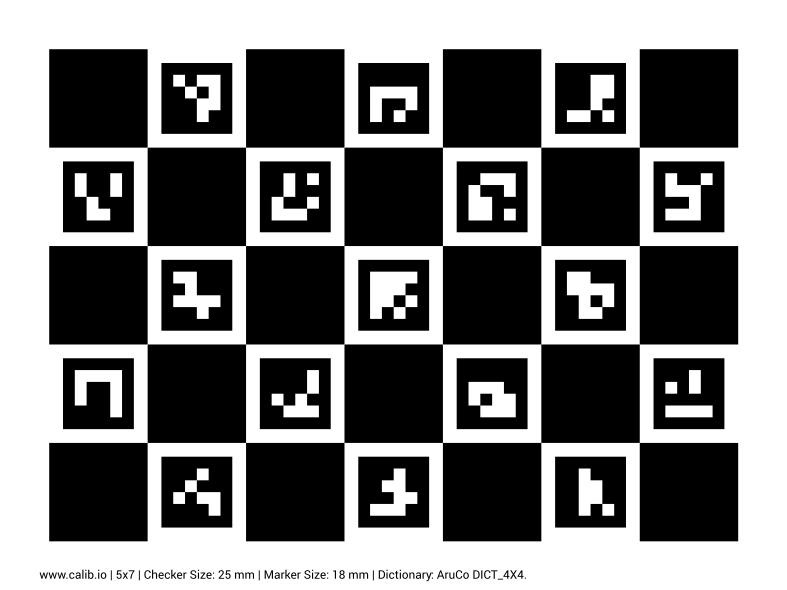
\includegraphics[width=0.7\textwidth]{figs/calib_io_charuco_200x150_5x7_25_18_DICT_4X4.png}
    \caption{ArUco marker for alignment of the digital twin}
    \label{f:aruco_marker}
    \end{subfigure}
        \hfill
    \begin{subfigure}[b]{0.45\textwidth}
        \centering
        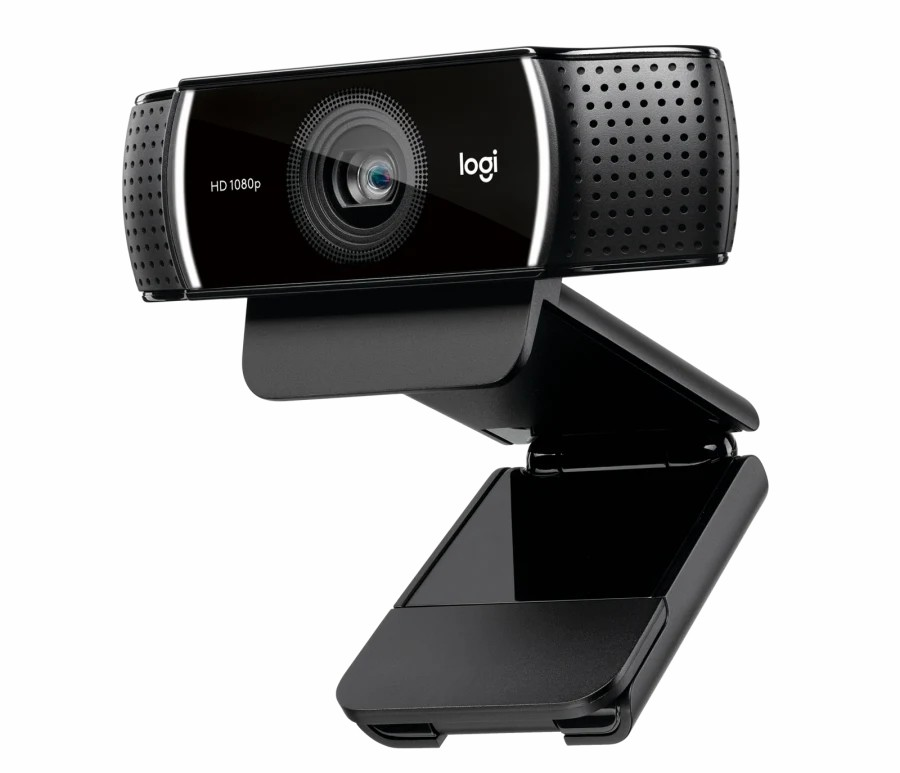
\includegraphics[width=0.7\linewidth]{figs/camera-c922.jpg}
        \caption{Logitech c922 camera used for marker detection}
        \label{fig:camera-c922}
    \end{subfigure}
    \caption{Marker and camera setup for digital and physical robot alignment}
\label{marker-camera}
\end{figure}

In Figure \ref{f:ur10_marker_unity} the digital robot model can be seen positioned realitve to the above described marker.

\begin{figure}[h]
    \centering
    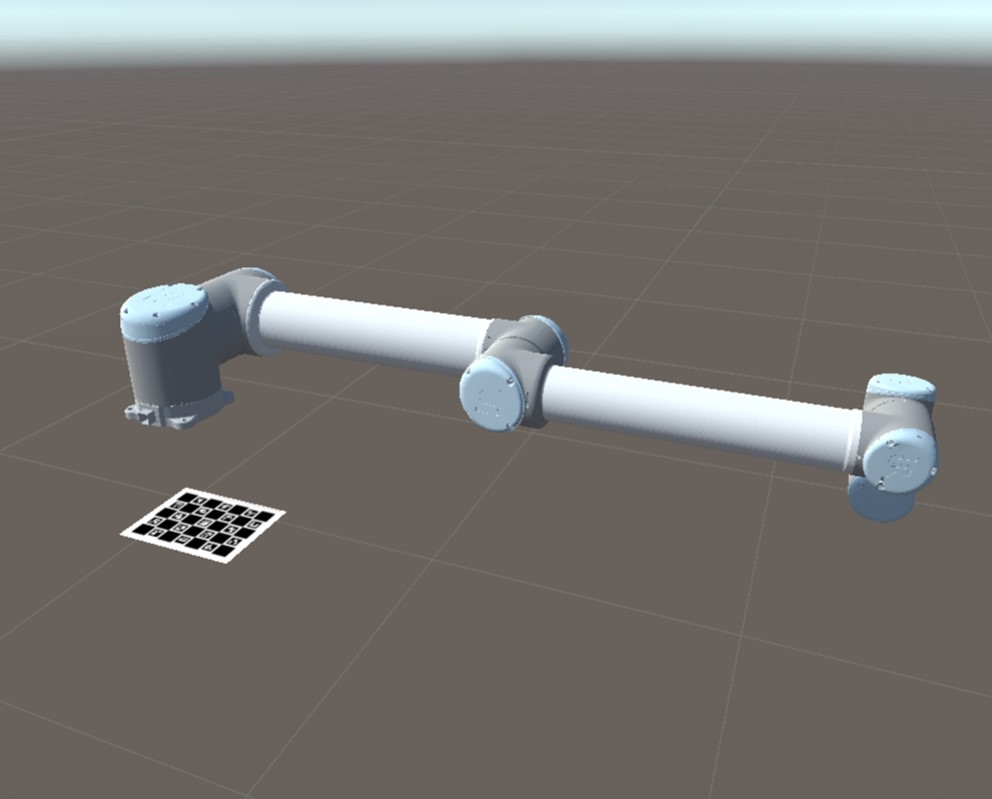
\includegraphics[width=0.6\textwidth]{figs/robot_marker_unity.jpg}
    \caption{Digital UR10 model aligned with ArUco marker in Unity}
    \label{f:ur10_marker_unity}
\end{figure}

* TODO: Add a figure showing the digital UR10 model aligned with the real ArUco marker and the real robot in the background. This will visually represent the alignment process.

\section{Bidirectional Communication}

After having the digital model correctly aligned with the physical robot, the next step was to establish bidirectional communication between the Unity and the UR10e. This communication was essential for enabling remote control of the physical robot through the \ac{DT}, as well as for synchronizing the robot's state between the real and virtual environments.

\subsection{ROS}

The Robot Operating System (\ac{ROS}) was chosen as the middleware for facilitating real-time communication between the physical robot and the Unity environment, since the UR10e robot from IRIS-LAB already had prior developed \ac{ROS} packages, such as \texttt{iris\_ur10e} \footnote{IRIS-LAB github Repository \url{https://github.com/iris-ua/iris_ur10e}, Acessed: 2024-02-02} and \texttt{iris\_sami} \footnote{IRIS-LAB github Repository for UR10e Robot Manipulation \url{https://github.com/iris-ua/iris_ur10e}, Acessed: 2024-02-02}.

These packages provided a comprehensive \ac{ROS} setup for controlling the UR10e robot, including trajectory planning, RViz visualization, and real-time operation. 
\ac{ROS} offers a robust and flexible framework for developing complex robotic systems. In this project, it enables seamless integration between hardware components and software modules. Specifically, \ac{ROS} facilitates the exchange of sensor data, control commands, and state information between the physical UR10e robot and its digital twin in Unity, ensuring synchronization for remote control and collaborative operations.


\section{Message Generation}
% \subsection{UR10e ROS Documentation}
% While Unity was chosen for its ability to create immersive environments, ROS (Robot Operating System) was selected to facilitate communication between the physical robot and its digital twin. The UR10e robot runs on ROS Noetic, which was configured on Ubuntu 20.04. By using ROS-TCP-Connector and ROS-TCP-Endpoint packages \footnote{Unity ROS Connector \url{https://github.com/Unity-Technologies/ROS-TCP-Connector} Accessed: 2024-02-02}

% a resume for each definition of the tools used in the implementation of the project - removeeeeeeeeeeeeeeeeeeee?
% Unity serves as the central development platform, integrating 3D models and real-time visualization to create the \ac{DT}. Vuforia, in conjunction with \ac{AR} markers, ensures precise pose registration between the physical robot and its digital counterpart. Additionally, \ac{ROS} (Robot Operating System) serves as the middleware facilitating real-time communication between the physical robot and the Unity environment. Together, these tools form the backbone of the system's functionality, enabling seamless collaboration between human operators and robotic systems in both physical and virtual spaces.
